\chapter{总体设计}
\section{软件描述}
%系统包括前台和后台两个部分。

%前台主要功能是:

%后台主要功能是:
系统包括客户端和服务端两个部分。

客户端为用户提供图形界面,用户可以在客户端上登陆账号,搜索添加好友,和好友聊天,参与群聊,发送语音视频消息。

服务端为客户端提供支持,存储用户数据和消息记录,在不同用户间转发聊天消息,提供搜索功能。

\section{处理流程}
\subsection{总体流程}
%此处应当有一个图和对应的描述。

\begin{figure}[h]
	\centering
	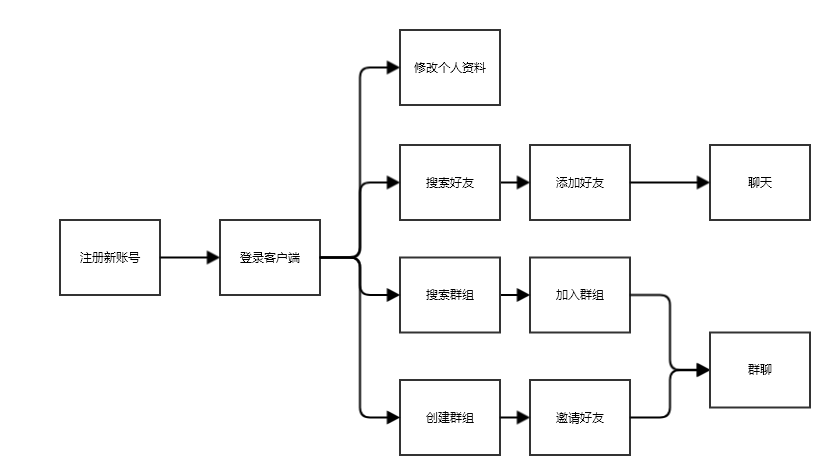
\includegraphics[width=13cm]{base_flowchart}
	\caption{总体流程图} \label{fig:base_flowchart}
\end{figure}

%\subsection{系统基本流程}
%此处应当有一个图和对应的描述。

\subsection{客户端基本流程}
%这只是举个例子,如果没有客户端则不需要此节。
\begin{figure}[h]
	\centering
	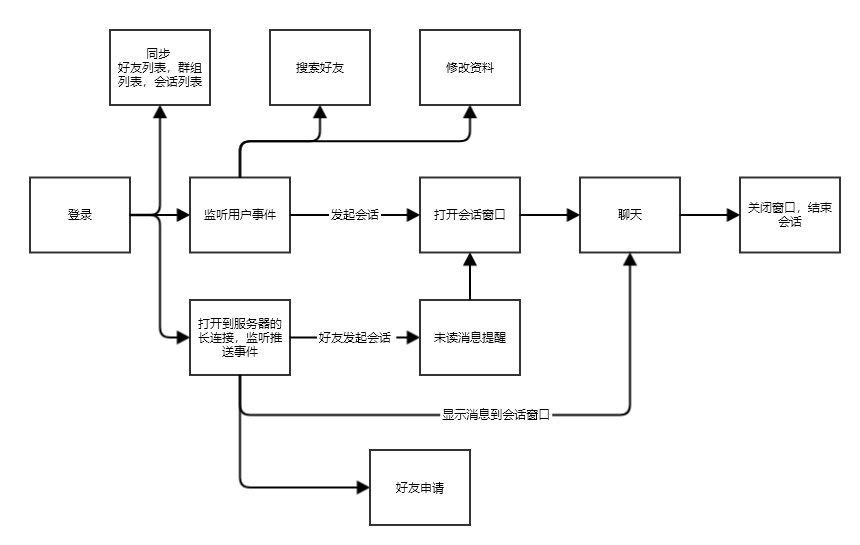
\includegraphics[width=13cm]{client_flowchart}
	\caption{客户端流程图} \label{fig:client_flowchart}
\end{figure}
用户在登陆账号后,客户端会从服务器同步好友,群组和会话信息。并打开一个到服务器的长连接,监听服务器的推送消息。
用户可以点击好友列表或群组列表中的项目启动一个会话窗口,在会话窗口中发送各种消息。
服务器会及时推送消息给客户端,客户端会将消息及时显示到对应的窗口中。
客户端也提供好友搜索,个人资料修改等功能。
见图-\ref{fig:client_flowchart}

\subsection{服务器端基本流程}
%这只是举个例子,如果没有服务器端则不需要此节。
\begin{figure}[h]
	\centering
	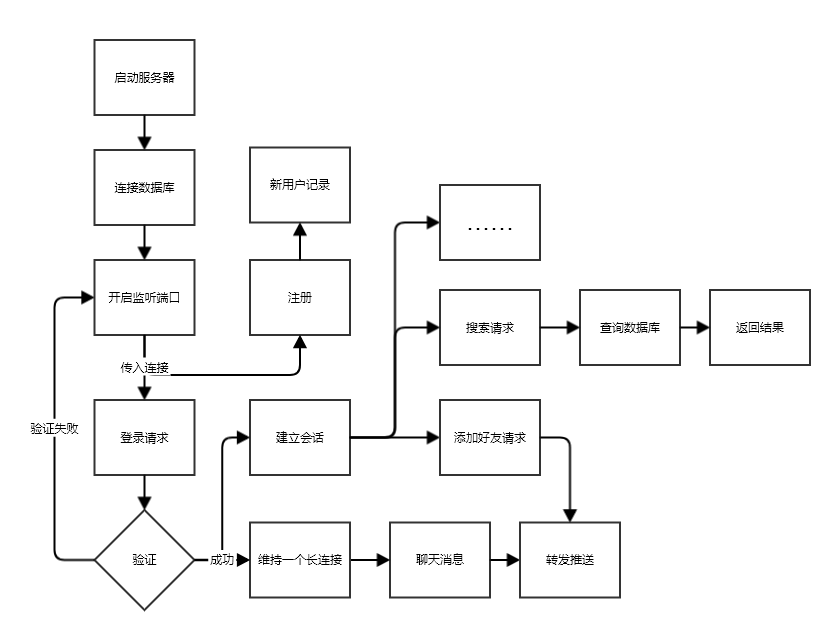
\includegraphics[width=13cm]{server_flowchart}
	\caption{服务端流程图} \label{fig:server_flowchart}
\end{figure}

服务端启动后连接数据库,监听端口,响应来自客户端的请求。
处理注册请求,验证合法后向数据库插入一条新纪录。
处理登陆请求,验证合法后为该账号分配一个 session 对象,
并维持一条到客户端的长连接,聊天消息,好友请求都会从该连接推送给客户端。
服务端亦提供 http api,用于修改个人资料,查找用户等功能。
见图-\ref{fig:server_flowchart}


\subsection{登录功能具体流程}
%此处应当有描述。
\begin{figure}[h]
	\centering
	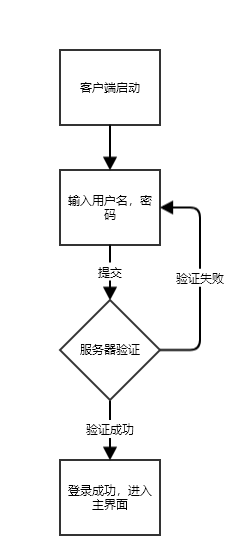
\includegraphics[width=5cm]{login_flowchart}
	\caption{登录功能流程图} \label{fig:login_flowchart}
\end{figure}
用户打开客户端,输入用户名和密码,点击登录提交至服务器,服务器查询数据库验证用户名密码是否合法。
若合法则进入主界面,否则提示用户出错。
见图-\ref{fig:login_flowchart}


\subsection{用户搜索功能具体流程}
%此处应当有一个描述。
\begin{figure}[h]
	\centering
	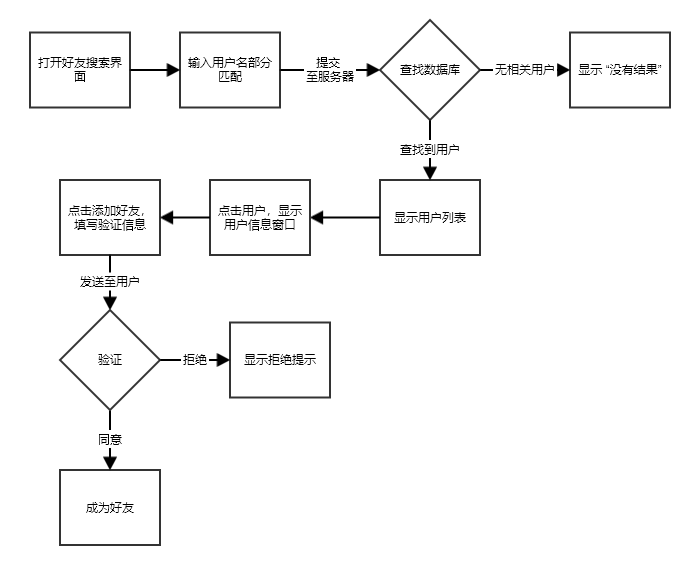
\includegraphics[width=13cm]{search_friend_flowchart}
	\caption{用户搜索功能流程图} \label{fig:search_friend_flowchart}
\end{figure}
用户打开搜索窗口,在搜索框输入要搜索的内容,一般是用户名的部分匹配。点击按钮提交给服务器。
服务器获取参数后查询数据库,获取返回结果,若无记录,则返回错误代码,客户端收到响应后显示无结果。
否则客户端将收到的用户数据以列表形式显示出来。
用户可以点击搜索结果中的项目打开用户信息窗口,添加好友。

\subsection{聊天功能具体流程}
用户在客户端的好友列表或群组列表选择项目,打开会话窗口,即可发送文本,图片或者语音消息。
消息数据会通过长连接发送给服务器。
服务器在接收到消息后就会推送给相应的用户。如果是群聊,则广播给所有群成员。
其他客户端收到后,若之前并未打开会话窗口,则会收到消息提醒。
若会话窗口已打开,则消息内容会显示到会话窗口中。
消息本身也将保存在服务器的数据库中。
不在线的用户上线后,服务器会推送未读的消息给客户端。

\section{功能结构设计}
\subsection{整体结构}
%此处应当有一个图和对应的描述。系统如果像微内核那样,划分成核心模块和若干个子系统,此处应当有图示及说明,然后后续几个节应当描述这几个子系统。如果系统像宏内核,那应当说明有哪些紧密联系的模块,并在后续几个节内描述这些模块。

\begin{figure}[h]
	\centering
	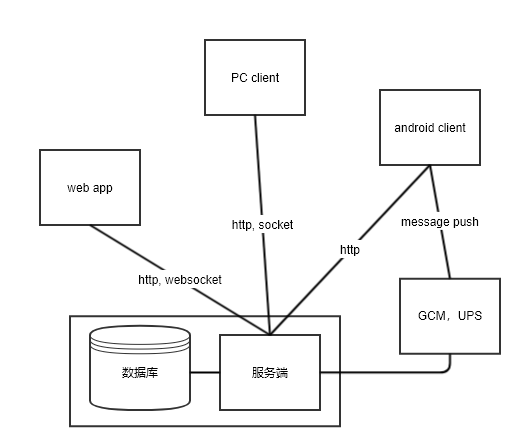
\includegraphics[width=13cm]{overall_architecture}
	\caption{整体结构} \label{fig:overall_architecture}
\end{figure}

\subsection{用户端结构}
% 此处应当有一个图和对应的描述。这只是举个例子。可能的内容包括用户端的具体模块、耦合情况等。


\subsection{服务器端结构}
% 此处应当有一个图和对应的描述。这只是举个例子。
\subsubsection{Django Web应用与Python运行时}
该模块是本Web系统的主要成分。

\subsubsection{Nginx}
该模块将作为前端服务器程序,处理所有到达服务器的请求(包括对静态资源的请求)。同时为Django应用提供反向代理。

\subsubsection{HTML/CSS模板和JS脚本}
为Web客户端界面提供模板、样式和必要的动画。由Nginx模块和Django Web应用读取,生成HTTP应答返回给用户。

\subsubsection{MySQL数据库}
该模块存储所有的用户、会话及其他数据。数据库会与Django Web应用以\href{https://www.python.org/dev/peps/pep-0249}{PEP 249}所定义的API进行通信。

\subsection{后台数据库维护模块结构}
此处应当有一个图和对应的描述。这只是举个例子。



\section{功能需求与程序代码的关系}
[此处指的是不同的需求分配到哪些模块去实现。可按不同的端拆分此表]
\begin{table}[htbp]
\centering
\caption{功能需求与程序代码的关系表} \label{tab:requirement-module}
\begin{tabular}{|c|c|c|c|}
    \hline
    · & 模块1 & 模块2 & 模块3 \\
    \hline
    需求1 & · & Y & · \\
    \hline
    需求2 & · & Y & · \\
    \hline
    需求3 & · & Y & · \\
    \hline
    需求4 & Y & · & · \\
    \hline
    需求5 & · & · & Y \\
    \hline
\end{tabular}
\note{各项功能需求的实现与各个程序模块的分配关系}
\end{table}